\newpage
\section{Resultados}

\subsection{Modulador série}

\begin{figure}[H]
	\centering
	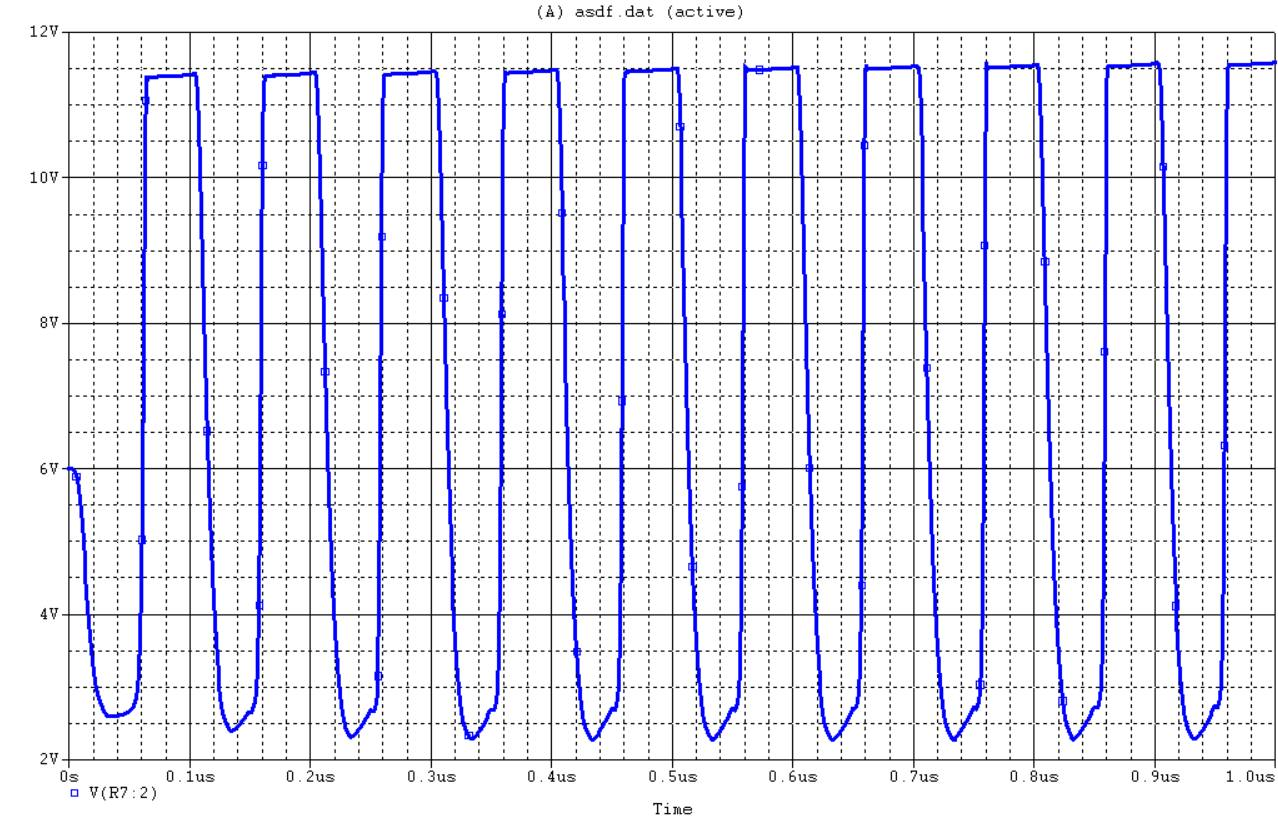
\includegraphics[scale=0.3]{Imagens/saida.jpg}
	\caption{Onda de saída para o oscilador a cristal.}
	\label{f_saida}
\end{figure}

\begin{figure}[H]
	\centering
	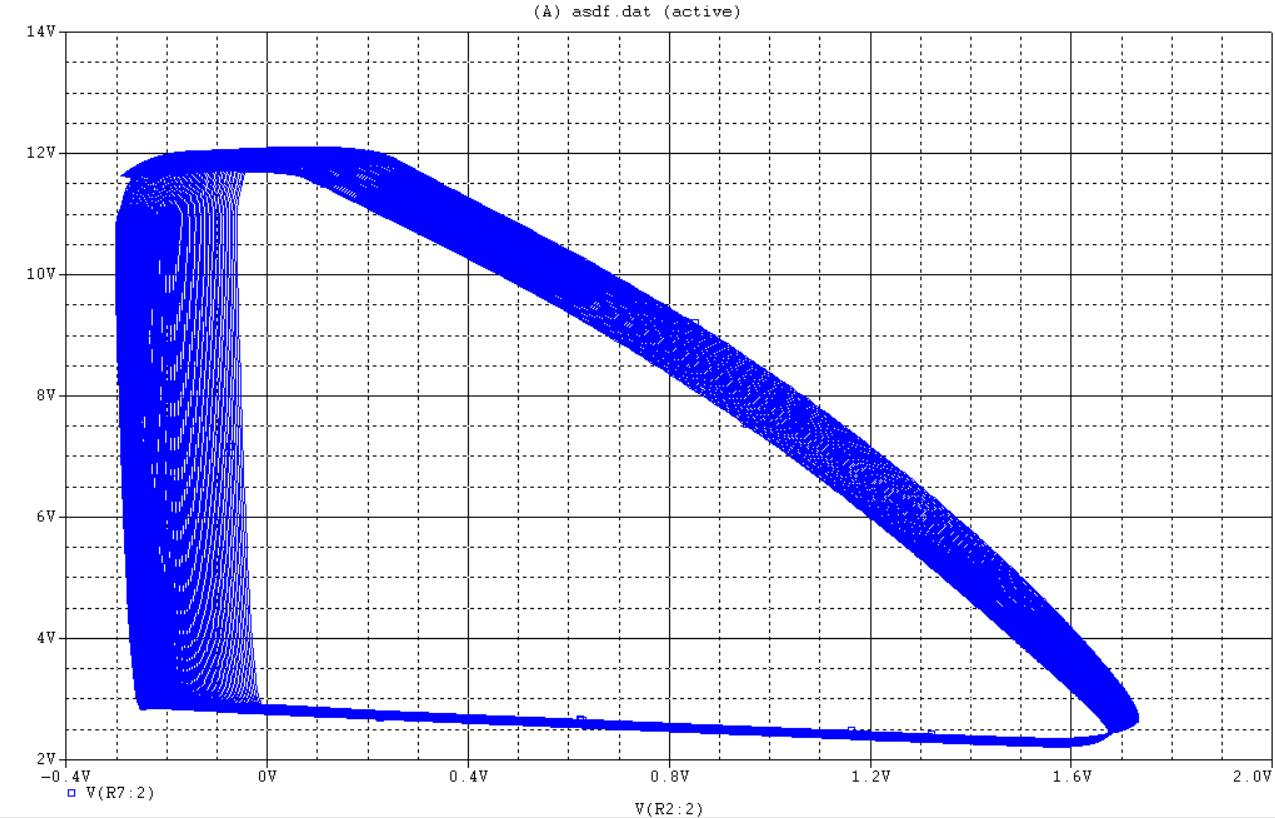
\includegraphics[scale=0.3]{Imagens/lissajous.jpg}
	\caption{Figura de lissajous.}
	\label{f_lissajous}
\end{figure}


\subsection{Modulador a diodo}
Após colocar a ponta de prova do osciloscópio, a frequência alterou para 10.01155MHz, mostrando que há uma pequena interferência no periodo do oscilador.